\section{Bench and Instruments}
\label{sec:method-bench}

The converter was supplied by the ITECH IT-M7723 programmable source. The
selected fixed output was connected to an ITECH IT8512+ electronic load or the
USB-C sink arrangement. A PC UART terminal was used to command the controller
and collect diagnostics. Load demand was set independently of the controller's
load estimate.

\begin{figure}[htbp]
\centering
\begin{subfigure}[t]{0.48\textwidth}
\centering
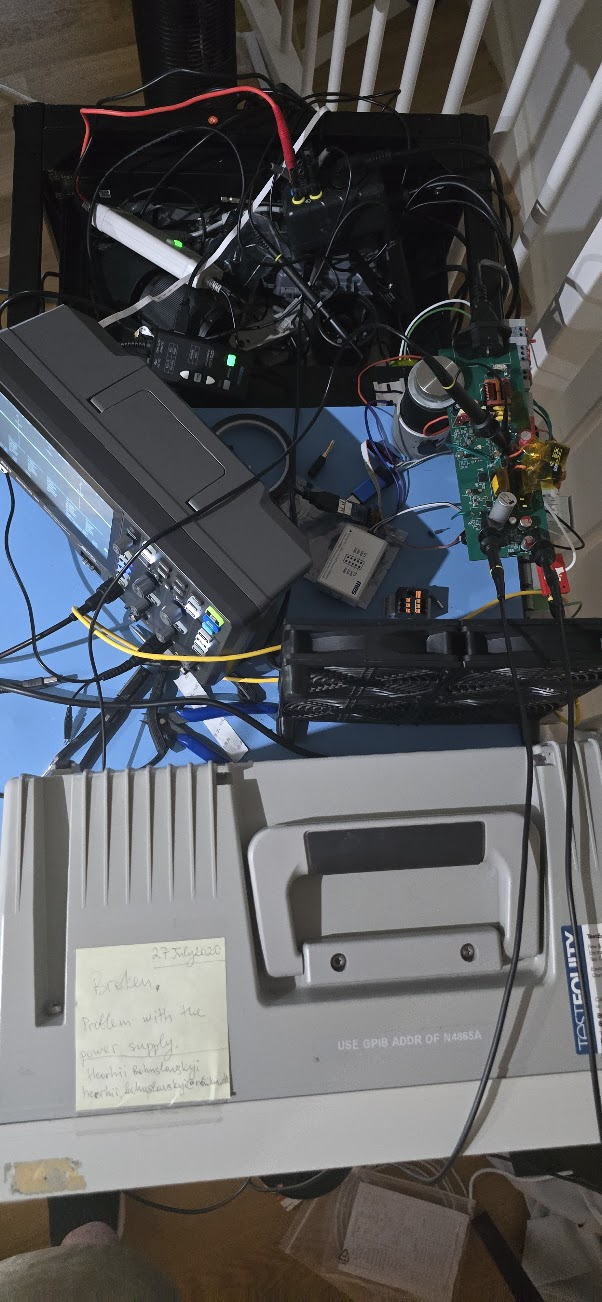
\includegraphics[width=\textwidth]{Pictures/Thesis/09_Methods/test_bench_overview_photo.png}
\caption{Source, load, and measurement arrangement.}
\label{fig:test-bench-overview-photo}
\end{subfigure}
\hfill
\begin{subfigure}[t]{0.48\textwidth}
\centering
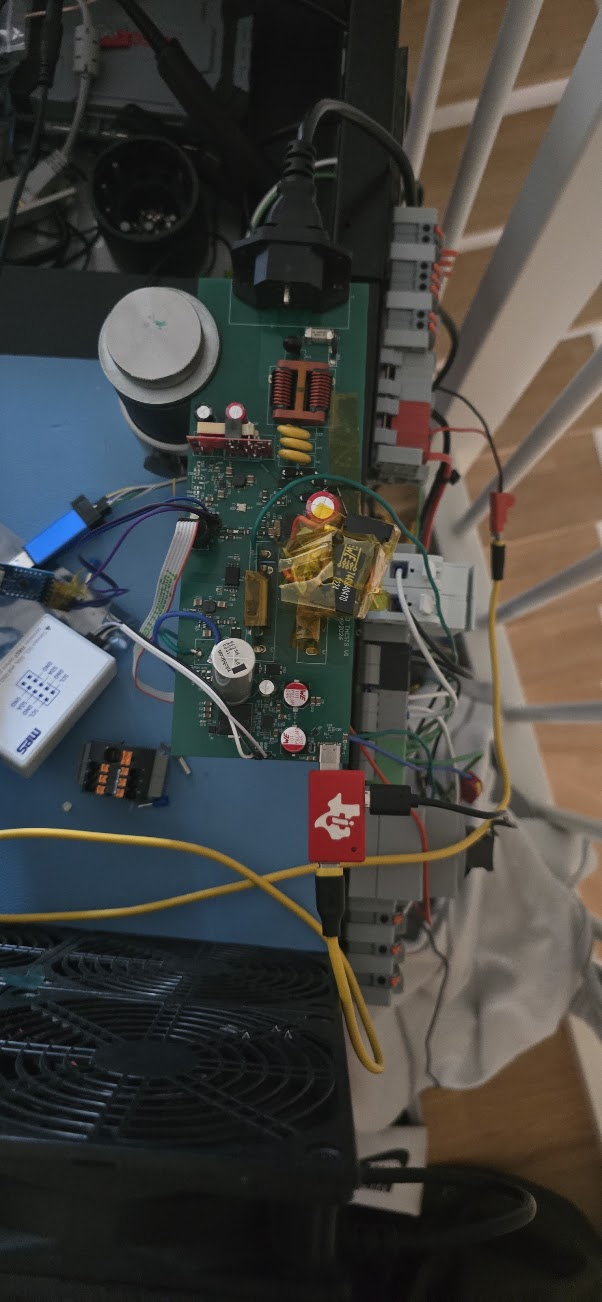
\includegraphics[width=\textwidth]{Pictures/Thesis/09_Methods/dut_probe_closeup_photo.png}
\caption{Probe access at the converter.}
\label{fig:dut-probe-closeup-photo}
\end{subfigure}
\caption{Test bench and probe connections.}
\label{fig:method-bench-photos}
\end{figure}

For input power and harmonics, the Siglent SDS824X HD was used with a Micsig
DP10013 differential voltage probe and CP2100A current probe. Switching and
output-voltage events were captured with the Keysight MSO9254A. The project
notes list February 2, 2026 as the calibration date for the main source, load,
oscilloscopes, and listed probes. Instrument serial numbers and calibration certificates
were not available.

\begin{table}[htbp]
\centering
\caption{Test equipment.}
\label{tab:bench-equipment}
\small
\begin{tabularx}{\textwidth}{@{}p{0.23\textwidth}p{0.34\textwidth}X@{}}
\toprule
Equipment & Model or range & Role\\
\midrule
Programmable source & ITECH IT-M7723 & Controlled AC input\\
Electronic load & ITECH IT8512+; \SI{120}{\volt}, \SI{30}{\ampere}, \SI{300}{\watt} & Steady and dynamic loading\\
Power-analysis oscilloscope & Siglent SDS824X HD & RMS, real power, PF, THD, and harmonics\\
Time-domain oscilloscope & Keysight MSO9254A & Switching and output events\\
Differential voltage probe & Micsig DP10013; \SI{100}{\mega\hertz}, 50X/500X & Input and high-voltage differential measurements\\
Current probe & Micsig CP2100A; DC--\SI{800}{\kilo\hertz} & Input or selected branch current\\
UART connection & \SI{115200}{baud} & Configuration, operating state, and firmware timing\\
\bottomrule
\end{tabularx}
\end{table}

Where practical, input power was measured at the DUT terminals, including
internally supplied auxiliaries. Output results identify the secondary-bulk,
connector-VBUS, or load-sense location; measurements beyond the cable include
its voltage drop and loss.
